\documentclass{scrartcl}
\usepackage{amsmath,amssymb,commath,graphicx}
\setkomafont{disposition}{\normalfont\bfseries}

\title{Mat 354}
\subtitle{Homework 2}
\author{Kenny Roffo}
\date{Due September 9, 2015}

\begin{document}
\maketitle
\textbf{1)} Use R to do the following with the data from Exercise 1.4 of the Mathematical Statistics text book.\\

\textbf{a.} Obtain a Histogram:\\
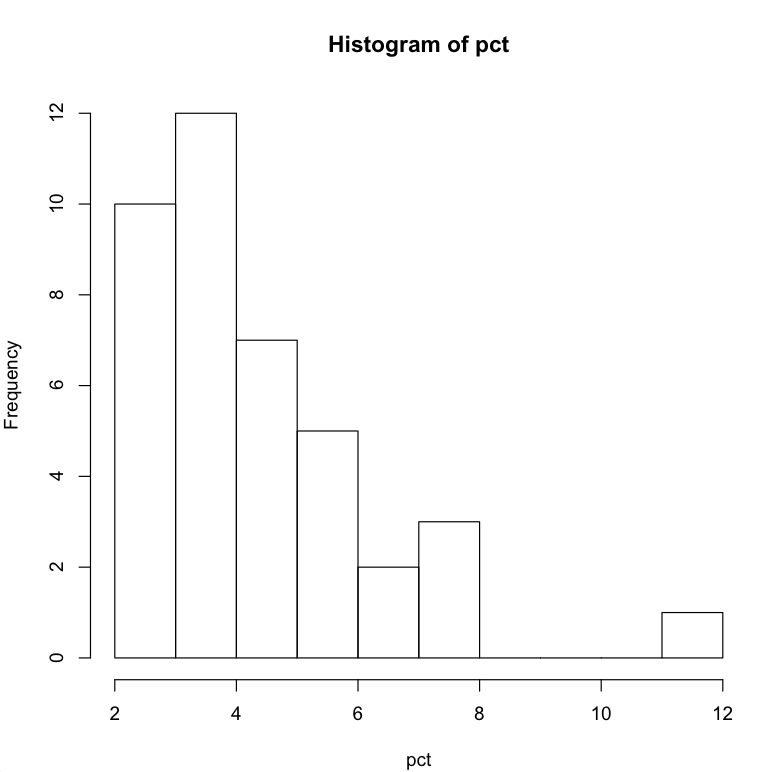
\includegraphics[keepaspectratio=true, scale=0.2]{1a.png}\\

\textbf{b.} Compute the mean and the standard deviation:\\
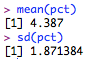
\includegraphics[keepaspectratio=true, scale=0.75]{1b.png}\\

\textbf{c.} Using the data (mine is pct) try assigning to a variable pct > 4 and printing the sum of that variable:\\
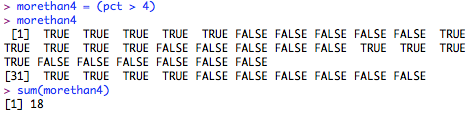
\includegraphics[keepaspectratio=true, scale=0.75]{1c.png}\\
Since the mean is close to 4, and 18 of 40 of the data points are above 4 (almost half) we can tell that the data set is probably symmetric without actually looking at it. The vector morethan4 holds the value true or false for each position depending on if the corresponding position in pct holds a value greater than 4. The way R handles statments such as pct > 4 is by creating a vector of the same length holding the values given by evaluating the statement on each individual index in pct. The sum of pct simply adds all the values. In R, TRUE and 1 are technically the same thing, and FALSE is 0, so the value returned is really just the number of values in the vector that were TRUE.

\textbf{d.} Delete the 11.88 from pct in R and find the mean and standard deviation again.\\
The suggested way to do this will work, however it will delete all values of 11.88. If there happen to be more in a future dataset then this may be an unwanted effect. To remove the $n^{th}$ element from the vector simply use pct[-n]. Here, 11.88 is the first element, so I will use pct[-1].
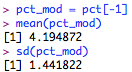
\includegraphics[keepaspectratio=true, scale=0.75]{1d.png}\\

\textbf{2)} Four random numbers between 1 and 10 (including the boundaries) are generated.\\

\textbf{a.} Determine the probability that the maximum is 5:\\
There are $10^4$ simple events which can occur (4 numbers with 10 possibilities for each). For the maximum of the 4 numbers to be 5, 3 of the numbers must be no greater than 5, and the remaining number must be 5. Let's say the first number is 5 (and 5 is the maximum). This event contains $1\cdot5^3$ elements (1 way to choose 5, 5 ways to choose a number less than or equal to 5 for the other 3 random numbers. Now consider when the second number is 5, the first number is strictly less than 5 (since we already counted when the first number is 5) and the remaining 2 are at most 5. This event contains $4\cdot1\cdot5^2$ elements. Now consider when the first 2 numbers are strictly less than 5, the third is 5 and the fourth is at most 5. This event contains $4^2\cdot1\cdot5$. Lastly, we have the event that the first 3 numbers are strictly less than 5 and the fourth is 5. This event has $4^3\cdot1$ elements. Note that these sets have been carefully chosen so that they are pairwise disjoint. Thus, the union of the sets (the event that the maximum of the numbers is 5) has cardinality equal to the cardinalities of the four sets created. This means there are $5^3+4\cdot5^2+4^2\cdot5+4^3$ elements in this event. Therefore, the probability that the maximum of the numbers is 5 is $\frac{5^3+4\cdot5^2+4^2\cdot5+4^3}{10^4}=0.0369$\\

\textbf{b.} Determine the probability that the minimum is no greater than 7.\\
Consider the event where the first number is less than or equal to 7. There are $7\cdot10^3$ elements of this event (7 ways to choose a number less than or equal to 7, and 10 ways to choose a number between 1 and 10). Now consider the event where the first number is greater than 7, and the second is at most 7. This event contains $3\cdot7\cdot10^2$ elements. Lastly consider the event where the first two numbers are greater than 7, and the third is at most 7, and the event where the first 3 numbers are greater than 7 and the fourth is at most 7. These events have $3^2\cdot7\cdot10$ and $3^3\cdot7$ elements respectively. Note that all of the events mentioned above are pairwise disjoint, thus union of these four sets (The event that the minimum is no greater than 7) has cardinality equal to the sum of their individual cardinalities. As a result, we now know that the probability that the minimum of the numbers is no greater than 7 is $\frac{7\cdot10^3+3\cdot7\cdot10^2+3^2\cdot7\cdot10+3^3\cdot7}{10^4}=0.9919$\\

\textbf{c.} Determine the probablity that the minimum is equal to 7.\\
Consider 4 pairwise disjoint events and their numbers of elements:
\begin{enumerate}
  \item The first number is 7, the other 3 are at least 7 \\ $1\cdot4^3$ elements
  \item The first number is at least 8, the second is 7 and the others are at least 7 \\ $3\cdot1\cdot4^2$ elements
  \item The first two numbers are at least 8, the third is 7 and the fourth is at least 7 \\ $3^2\cdot1\cdot4$elements
  \item The first three numbers are at least 8 and the fourth is 7 \\ $3^3\cdot1$ elements
\end{enumerate}
The event made from the union of these events is the event that the minimum of the numbers is 7, and has cardinality equal to the sum of the cardinalities of these sets. Therefore, the probability that the minimum of the numbers is equal to 7 is $\frac{4^3+3\cdot4^2+3^2\cdot4+3^3}{10^4}=0.0175$\\

\textbf{3)} Alter the 4-integer problem so that the integers are chosen from a simple random sample.\\

\textbf{a.} Determine the probability that the maximum is 8.
The first number can be any number less than 9, so there are 8 possibilities for the first number. Once this number is generated, it cannot be generated again, so for the second number to be at most 8 there are $8-1=7$ possibilities. Likewise there are 6 and 5 ways to choose the third and fourth numbers respectively such that they are at most 8. Thus there are $8\cdot7\cdot6\cdot5$ elements in the event that the maximum value is 8, so the probability of this event occurring is $\frac{8\cdot7\cdot6\cdot5}{10\cdot9\cdot8\cdot7}=\frac{1}{3}$\\

\textbf{b.} Determine the probability that the minimum is 8.\\
Since a simple random sample has no replacement, it is impossible to have the minimum value be 8. There are only 3 numbers to choose from which are not less than 8 (8, 9 and 10), but we must get 4 numbers, so the minimum value can at most be 7. Therefore the probability that the minimum is 8 is 0.
\end{document}

